%%%%%%%%%%%%%%%%%%%%%%%%%%%%%%%%%%%%%%%%%%%%%%%%%%%%%%%%%%%%%%%%%%%%
%% I, the copyright holder of this work, release this work into the
%% public domain. This applies worldwide. In some countries this may
%% not be legally possible; if so: I grant anyone the right to use
%% this work for any purpose, without any conditions, unless such
%% conditions are required by law.
%%%%%%%%%%%%%%%%%%%%%%%%%%%%%%%%%%%%%%%%%%%%%%%%%%%%%%%%%%%%%%%%%%%%

\documentclass{beamer}
\usetheme[faculty=phil]{fibeamer}
\usepackage[utf8]{inputenc}
\usepackage[
  main=english, %% By using `czech` or `slovak` as the main locale
                %% instead of `english`, you can typeset the
                %% presentation in either Czech or Slovak,
                %% respectively.
  czech, slovak %% The additional keys allow foreign texts to be
]{babel}        %% typeset as follows:
%%
%%   \begin{otherlanguage}{czech}   ... \end{otherlanguage}
%%   \begin{otherlanguage}{slovak}  ... \end{otherlanguage}
%%
%% These macros specify information about the presentation
\title{Classical Black Holes} %% that will be typeset on the
\subtitle{04. Rotating Black Holes} %% title page.
\author{Edward Larra\~{n}aga}
%% These additional packages are used within the document:
\usepackage{ragged2e}  % `\justifying` text
\usepackage{booktabs}  % Tables
\usepackage{tabularx}
\usepackage{tikz}      % Diagrams
\usetikzlibrary{calc, shapes, backgrounds}
\usepackage{amsmath, amssymb}
\usepackage{url}       % `\url`s
\usepackage{listings}  % Code listings
\usepackage{siunitx}
\frenchspacing
\begin{document}
  \frame{\maketitle}

  \AtBeginSection[]{% Print an outline at the beginning of sections
    \begin{frame}<beamer>
      \frametitle{Outline for Part \thesection}
      \tableofcontents[currentsection]
    \end{frame}}
    \section{The Rotating Black Hole in General Relativity}
    
    \subsection{The Rotating Black Hole in General Relativity}
    	\begin{frame}{Kerr's Solution}
    		Boyer-Lindquist coordinates: $\left(t,r,\theta,\varphi\right)$
            \pause
            \begin{align*}
            ds^{2} &= -\frac{\Delta-a^{2}\sin^{2}\theta}{\varrho}dt^{2}-\left(\frac{r^{2}+a^{2}-\Delta}{\varrho}\right)2a\sin^{2}\theta dtd\varphi\nonumber \\
             & +\frac{\varrho}{\Delta}dr^{2}+\varrho d\theta^{2}+\left(\frac{\left(r^{2}+a^{2}\right)^{2}-\Delta a^{2}\sin^{2}\theta}{\varrho}\right)\sin^{2}\theta d\varphi^{2}.
            \end{align*}
            \pause
            $$\varrho  = r^{2}+a^{2}\cos^{2}\theta$$
            $$\Delta =  r^{2}-2Mr+a^{2}$$
    	\end{frame}

	\subsection{The Kerr-Newman Family}
         \begin{frame}{The Kerr-Newman Family}
            \begin{align*}
			ds^{2} &= -\frac{\Delta-a^{2}\sin^{2}\theta}{\varrho}dt^{2}-\left(\frac{r^{2}+a^{2}-\Delta}{\varrho}\right)2a\sin^{2}\theta dtd\varphi\nonumber \\
 & +\frac{\varrho}{\Delta}dr^{2}+\varrho d\theta^{2}+\left(\frac{\left(r^{2}+a^{2}\right)^{2}-\Delta a^{2}\sin^{2}\theta}{\varrho}\right)\sin^{2}\theta d\varphi^{2}
			\end{align*}

			\begin{align*}
            \varrho &=  r^{2}+a^{2}\cos^{2}\theta\\
            \Delta &=  r^{2}-2Mr+a^{2}+e^{2}
            \end{align*}
        \end{frame}
        
        \begin{frame}{The Kerr-Newman Family}
            $$a=\frac{J}{M}$$
			$$e=\sqrt{Q^{2}+P^{2}}$$
			$Q$: Electric charge\\
            $P$: Magnetic monopole charge\\
            The electromagnetic 4-potential is
			$$A=\frac{Qr\left[dt-a\sin^{2}\theta d\varphi\right]-P\cos\theta\left[adt-\left(r^{2}+a^{2}\right)d\varphi\right]}{\varrho}$$
        \end{frame}
        
        \begin{frame}{Kerr's Solution}
            \begin{align*}
            ds^{2} &= -\frac{\Delta-a^{2}\sin^{2}\theta}{\varrho}dt^{2}-\left(\frac{r^{2}+a^{2}-\Delta}{\varrho}\right)2a\sin^{2}\theta dtd\varphi\nonumber \\
             & +\frac{\varrho}{\Delta}dr^{2}+\varrho d\theta^{2}+\left(\frac{\left(r^{2}+a^{2}\right)^{2}-\Delta a^{2}\sin^{2}\theta}{\varrho}\right)\sin^{2}\theta d\varphi^{2}.
            \end{align*}
            $$\varrho  = r^{2}+a^{2}\cos^{2}\theta$$
            $$\Delta =  r^{2}-2Mr+a^{2}$$
            $$a=\frac{J}{M}$$
    	\end{frame}

	\subsection{Killing Vectors}
        \begin{frame}{Killing Vectors}
        	\pause
            $$\xi  =  \frac{\partial}{\partial t}$$
			Asymptotically timelike vector
            \pause
			$$\zeta=\frac{\partial}{\partial\varphi}$$
			Asymptotically spacelike vector
    	\end{frame}

	\subsection{Singularities}
        \begin{frame}{Kerr Black Hole Singularities}
            $$\varrho  = r^{2}+a^{2}\cos^{2}\theta = 0$$
            $$\Delta =  r^{2}-2Mr+a^{2} = 0$$
    	\end{frame}
        
        \begin{frame}{Kerr Black Hole Singularities}
            $$\varrho  = r^{2}+a^{2}\cos^{2}\theta = 0$$
            \pause
            \begin{eqnarray*}
            r=0 & , & \theta=\frac{\pi}{2}
            \end{eqnarray*}
            \pause
            This is an \textit{essential singularity} as is probed by the Kretschmann scalar,
            \pause
            $$ K = \frac{48M^2}{\varrho^6} \left[ r^6 - 15a^2 r^4 \cos^2\theta + 15a^4 r^2 \cos^4\theta - a^6 \cos^6 \theta \right] $$
    	\end{frame}
        
        \begin{frame}{Kerr Black Hole Singularities}
            $$\Delta =  r^{2}-2Mr+a^{2} = 0$$
            \pause
            $$\Delta = \left( r-r_{+} \right) \left( r-r_{-} \right) = 0 $$
            $$r_{\pm}=M\pm\sqrt{M^{2}-a^{2}}$$
            \pause
            These are \textit{coordinate singularities}
    	\end{frame}

	\subsection{Eddington-Finkelstein Coordinates}
        \begin{frame}{Eddington-Finkelstein Coordinates}
        	$$ (t, r, \theta, \phi) \longrightarrow (v, r, \theta, \chi) $$
            \pause
            $$ dv =  dt+\frac{\left(r^{2}+a^{2}\right)}{\Delta}dr$$
			$$ d\chi  =  d\varphi+\frac{a}{\Delta}dr$$
            \pause
        	\begin{align*}
ds^{2} & = -\frac{\Delta-a^{2}\sin^{2}\theta}{\varrho}dv^{2}+2dvdr-\frac{2a\sin^{2}\theta\left(r^{2}+a^{2}-\Delta\right)}{\varrho}dvd\chi\nonumber \\
 &  -2a\sin^{2}\theta drd\chi+\varrho d\theta^{2}+\frac{\left(r^{2}+a^{2}\right)^{2}-\Delta a^{2}\sin^{2}\theta}{\varrho}\sin^{2}\theta d\chi^{2}
\end{align*}
    	\end{frame}
        

	\subsection{Kerr Black Hole Cases}
    	\begin{frame}{Kerr Black Hole Singularities}
            $$r_{\pm}=M\pm\sqrt{M^{2}-a^{2}}$$
    	\end{frame}
       
        \begin{frame}{Case I: $M<a$}
            \begin{itemize}
            \item Both roots $r_{\pm}$ are complex
            \pause
            \item $\Delta$ has no real zeros 
            \pause
            \item There are no coordinate singularities
            \pause
            \item The essential singularity $\varrho=0$ exists
            \end{itemize}
        \end{frame}
        
    	\begin{frame}{Kerr-Schild's Coordinates}
        \framesubtitle{Case I: $M<a$}
            Kerr-Schild's coordinates: $\left(\tilde{t},x,y,z\right)$
            \pause
            \begin{eqnarray*}
            \tilde{t} & = & \int\left[dt+\frac{r^{2}+a^{2}}{\Delta}dr\right]-r\\
            x+iy & = & \left(r+ia\right)\sin\theta e^{i\int\left[d\varphi+\frac{a}{\Delta}dr\right]}\\
			z & = & r\cos\theta
			\end{eqnarray*}
        \end{frame}
        
		\begin{frame}{Kerr-Schild's Coordinates}
        \framesubtitle{Case I: $M<a$}
         	\begin{align*}
         	ds^{2} = &-d\tilde{t}^{2}+dx^{2}+dy^{2}+dz^{2} \\
  			&+\frac{2Mr^{3}}{r^{4}+a^{2}z^{2}}\left[\frac{r\left(xdx+ydy\right)-a\left(xdx-ydy\right)}{r^{2}+a^{2}}+\frac{zdz}{r}+d\tilde{t}^{2}\right]^{2}
 			\end{align*}
            \pause
            \bigskip
            
            $M=0$: Kerr's becomes Minkowski's space.
      	\end{frame}
        
        \begin{frame}{Kerr-Schild's Coordinates}
        \framesubtitle{Case I: $M<a$}
			$r=\mbox{constant}\neq0$ gives
$$\frac{x^{2}}{r^{2}}+\frac{y^{2}}{r^{2}}+\left(1+\frac{a^{2}}{r^{2}}\right)\frac{z^{2}}{r^{2}}=1+\frac{a^{2}}{r^{2}}$$
			\pause
            \begin{itemize}
            \item Ellipsoids with foci at $x=\pm a$
            \item These ellipsoids degenerate into the disk $\left\{ z=0,x^{2}+y^{2}\leq a^{2}\right\} $ for $r=0$
            \end{itemize}
        \end{frame}
        
        \begin{frame}{The Essential Singularity in Kerr-Schild's Coordinates}
        \framesubtitle{Case I: $M<a$}
			Essential singularity of Kerr's metric: $\varrho=0$
            \pause
			\begin{eqnarray*}
            r=0 & , & \theta=\frac{\pi}{2}
            \end{eqnarray*}            
            \pause
			$$x^{2}+y^{2}=a^{2}$$
            \pause
            \centering{Ring with radius $a$ centered at the origin}
        \end{frame}
        
        \begin{frame}{Surfaces of $r=\textrm{constant}$ in Kerr's metric}
        \framesubtitle{Case I: $M<a$}
        	\begin{center}
				\begin{figure}
				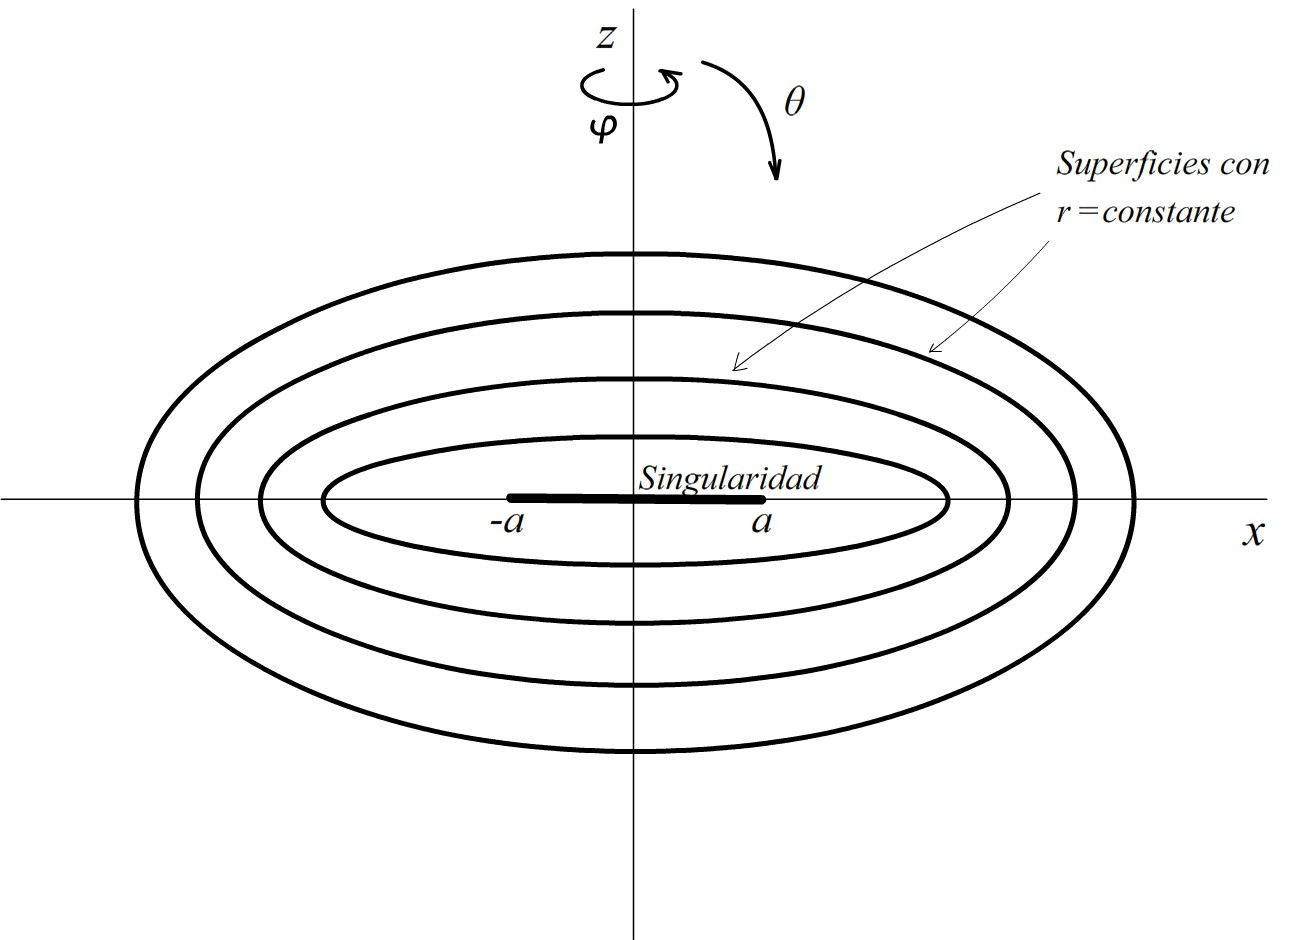
\includegraphics[scale=0.75] {figures/fig35.jpg}
				\end{figure}
			\end{center}	
        \end{frame}
        
        
        \begin{frame}{Carter-Penrose Diagram. $\theta=\frac{\pi}{2}$}
        \framesubtitle{Case I: $M<a$}
        	\begin{center}
				\begin{figure}
				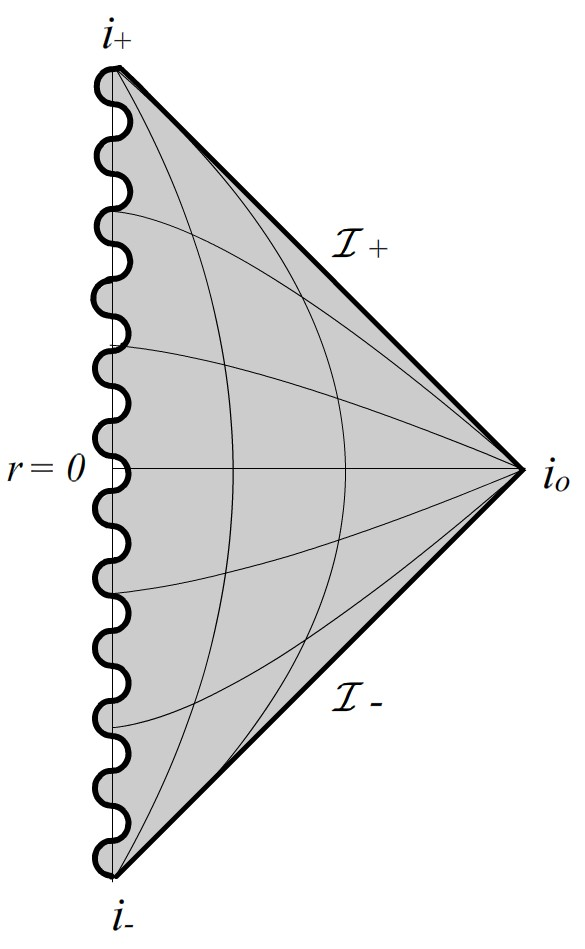
\includegraphics[scale=0.75] {figures/fig36.jpg}
				\end{figure}
			\end{center}	
        \end{frame}
        
      \begin{frame}{Carter-Penrose Diagram. $\theta=0$}
      \framesubtitle{Case I: $M<a$}
        	\begin{center}
				\begin{figure}
				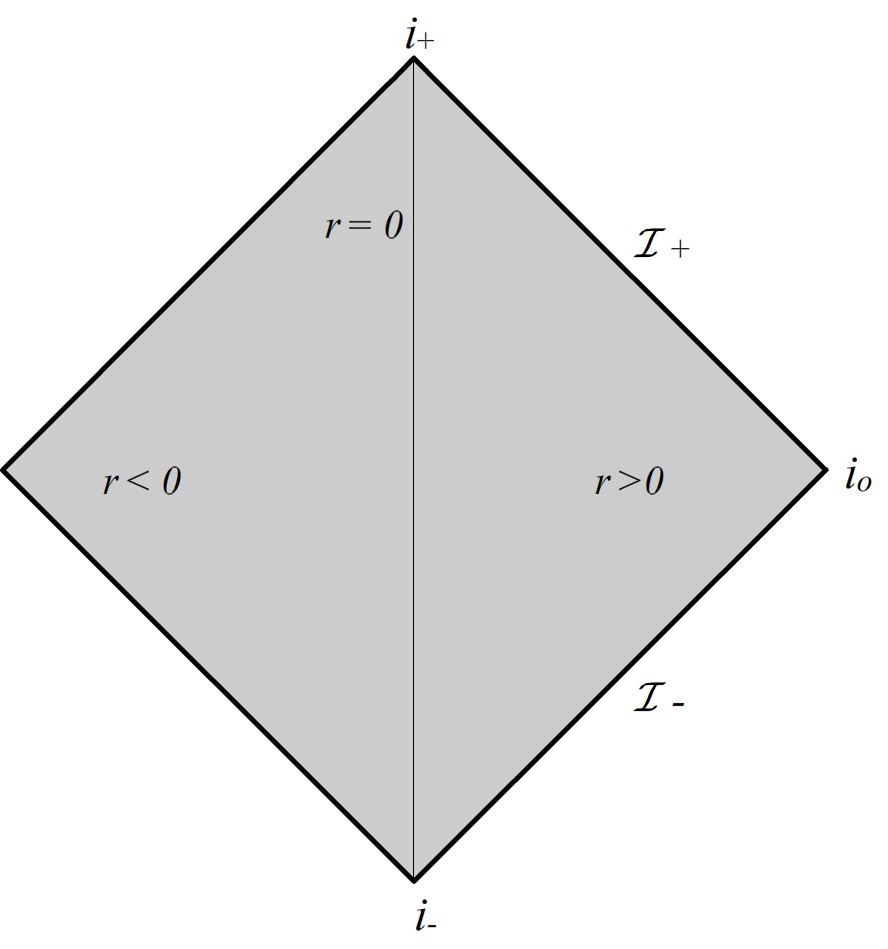
\includegraphics[scale=0.75] {figures/fig37.jpg}
				\end{figure}
			\end{center}	
        \end{frame}
    
        \begin{frame}{Causal Structure near the Singularity}
         \framesubtitle{Case I: $M<a$}
			\begin{itemize}
			\item The cosmic censorship hypotesis rules out the Case 1 of Kerr's metric
            	\pause
             \item Another reason to consider it as non-physical is the Causal structure near the essential singularity.
			\end{itemize}
        \end{frame}
        
 		\begin{frame}{Causal Structure near the Singularity}
         \framesubtitle{Case I: $M<a$}
			$$\zeta=\frac{\partial}{\partial\varphi}$$
            \centering{This vector field has closed orbits}
            \pause
            $$\zeta^{2}=g_{\mu\nu}\zeta^{\mu}\zeta^{\nu}=g_{\varphi\varphi}$$
            \pause
            $$\zeta^{2}=\left(\frac{\left(r^{2}+a^{2}\right)^{2}-\Delta a^{2}\sin^{2}\theta}{\varrho}\right)\sin^{2}\theta$$
        \end{frame}
        
        \begin{frame}{Causal Structure near the Singularity}
         \framesubtitle{Case I: $M<a$}
            In the neighborhood of the ring singularity:$\frac{r}{a}=\delta<<1$
and $\theta=\frac{\pi}{2}$
			\pause
			$$\zeta^{2}=a^{2}+\frac{Ma}{\delta}+O\left(\delta^{2}\right)$$
            \pause
            For points near the singularity in the region with negative
$r$, we have $\delta<0$.\\
			\pause
			The Killing vector may have a negative magnitude, $\zeta^{2}<0,$ i.e. it can be timelike.\\
        \end{frame}
        
        \begin{frame}{Causal Structure near the Singularity}
         \framesubtitle{Case I: $M<a$}
            Since $\xi$ has closed orbits, this fact permit the existence of closed timelike curves.\\
            \pause
            Violation of Causality!
        \end{frame}
        
        \begin{frame}{Kerr Black Hole Singularities}
            $$r_{\pm}=M\pm\sqrt{M^{2}-a^{2}}$$
    	\end{frame}
       
        \begin{frame}{Case II: $M>a$}
            \begin{itemize}
            \item The essential ring singularity $\varrho=0$ is dressed
with the coordinate singularities at $r=r_{\pm}$ 
            \pause
            \item The function $\Delta$ is positive for $r>r_{+}$ and $r<r_{-}$, but it is negative for $r_{-}<r<r_{+}$ 
            \pause
            \item The double change in sign makes the singularity $r=0$ timelike, just as in case I.
            \end{itemize}
        \end{frame}
        
        \begin{frame}{Killing Horizons}
         \framesubtitle{Case II: $M>a$}
            The hypersurfaces $r=r_{\pm}$ are Killing horizons of the Killing vector fields 
			$$\mathbf{\psi_{\pm}}=\frac{\partial}{\partial v}+\left(\frac{a}{r_{\pm}^{2}+a^{2}}\right)\frac{\partial}{\partial\chi}$$
        \end{frame}
        
        \begin{frame}{Killing Horizons}
         \framesubtitle{Case II: $M>a$}
            $$\Phi_{\pm}=r-r_{\pm}$$
            \pause
            $\Phi_{\pm}=0$ corresponds to the hypersurfaces $r=r_{\pm}$. 
            \pause
            \bigskip
            
            Normal vectors:
			$$\mathbf{n}_{\pm} =  N_{\pm}g^{\mu\nu}\partial_{\mu}\Phi\partial_{\nu}$$
            \pause
            $$\mathbf{n}_{\pm} = N_{\pm} \left[g^{rr}\partial_{r}+g^{rv}\partial_{v}+g^{r\chi}\partial_{\chi}\right]$$
        \end{frame}
        
        \begin{frame}{Killing Horizons}
         \framesubtitle{Case II: $M>a$}
            \begin{equation*}
            \begin{array}{lcl}
            g^{vv}=\frac{a^{2}\sin^{2}\theta}{\varrho} & \qquad & g^{vr}=\frac{a^{2}+r^{2}}{\varrho}\\
            g^{v\chi}=\frac{a}{\varrho} & \qquad & g^{r\chi}=\frac{a}{\varrho}\\
            g^{rr}=\frac{\Delta}{\varrho} & \qquad & g^{\theta\theta}=\frac{1}{\varrho}\\
            g^{\chi\chi}=\frac{\csc^{2}\theta}{\varrho} & \qquad
            \end{array}
            \end{equation*}
            \pause

            $$ \mathbf{n}_{\pm} = \frac{N_{\pm}}{\varrho}\left[\Delta\partial_{r}+\left(a^{2}+r^{2}\right)\partial_{v}+a\partial_{\chi}\right]$$        
        \end{frame}
        
        \begin{frame}{Killing Horizons}
         \framesubtitle{Case II: $M>a$}
        	Magnitude of the normal vector
            \footnotesize
            \begin{eqnarray*}
\mathbf{n}_{\pm}^{2} & =\frac{N_{\pm}^{2}}{\varrho^{2}} & \left[-\left(\frac{\Delta-a^{2}\sin^{2}\theta}{\varrho}\right)\left(a^{2}+r^{2}\right)^{2}+\frac{\left(r^{2}+a^{2}\right)^{2}-\Delta a^{2}\sin^{2}\theta}{\varrho}a^{2}\sin^{2}\theta\right.\nonumber \\
 &  & \left.+2\Delta\left(a^{2}+r^{2}\right)-\frac{2a^{2}\sin^{2}\theta\left(r^{2}+a^{2}-\Delta\right)}{\varrho}\left(a^{2}+r^{2}\right)-2a^{2}\Delta\sin^{2}\theta\right]
			\end{eqnarray*}
            \pause
            \normalsize
            At $r=r_{\pm}$ we have
            $$\left.\mathbf{n}_{\pm}^{2}\right|_{r=r_{\pm}}=0$$
            \pause
            i.e. these are null hypersurfaces.
       	\end{frame}
 
  		\begin{frame}{Killing Horizons}
         \framesubtitle{Case II: $M>a$}
  			Evaluating the normal vector at $r=r_{\pm}$ gives
            $$\left. \mathbf{n}_{\pm} \right|_{r=r_{\pm}} = N_{\pm}\left(\frac{a^{2} + r_{\pm}^{2}}{r_{\pm}^{2}+a^{2} \cos^{2}\theta} \right) \psi_{\pm}$$
  		\end{frame}
        
    	\begin{frame}{Surface Gravity}
         \framesubtitle{Case II: $M>a$}
			$$\left.n^{\sigma} \nabla_{\sigma} n^{\mu} \right|_{\mathcal{N}} = 0$$
 		\pause
        $$ \left.\xi^{\sigma} \nabla_{\sigma} \xi^{\mu}\right|_{\mathcal{N}} = \kappa\xi^{\mu}$$
        \pause
        $$\kappa_{\pm}=\frac{r_{\pm}-r_{\mp}}{2\left(a^{2}+r_{\pm}^{2}\right)}$$
    	\end{frame}
        
    	
        
        
        \begin{frame}{Carter-Penrose Diagram. $\theta=\frac{\pi}{2}$ and $\theta=0$}
         \framesubtitle{Case II: $M>a$}

        	\begin{center}
				\begin{figure}
				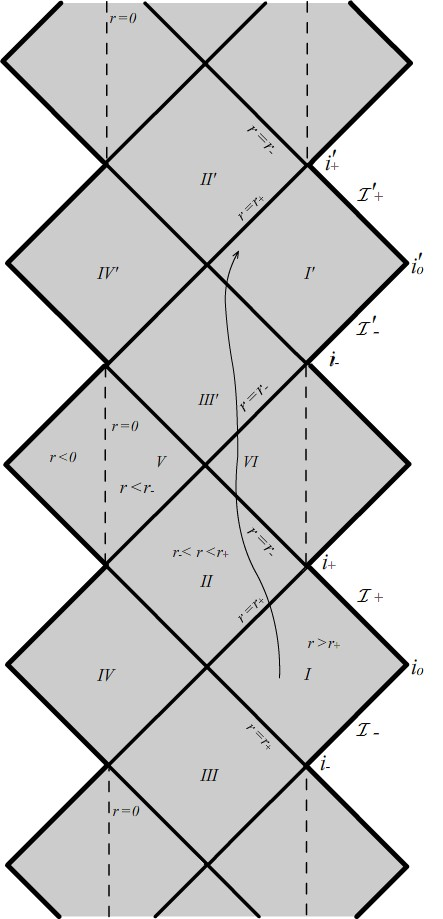
\includegraphics[scale=0.75] {figures/fig38.jpg}
				\end{figure}
			\end{center}	
        \end{frame}


	\section{Physical Properties of Kerr's Solution}    
  	\begin{darkframes}
        
        \subsection{Angular Velocity of the Black Hole}
        \begin{frame}{Angular Velocity of the Black Hole}
        \framesubtitle{Case II: $M>a$}
        The Killing vector $\psi_{+}$ in Boyer-Lindquist's coordinates is
		$$\psi_{+}=\frac{\partial}{\partial t}+\Omega\frac{\partial}{\partial\varphi}$$
		where 
		$$\Omega=\frac{a}{a^{2}+r_{+}^{2}}$$
        \end{frame}
        
        \begin{frame}{Angular Velocity of the Black Hole}
       	\framesubtitle{Case II: $M>a$}
        	$$\psi_{+}^{\mu}\partial_{\mu}\left[\varphi-\Omega t\right] = 0$$
            \pause
            Orbits of this Killing vector $\psi_{+}$:
            $$\varphi-\Omega t=\textrm{constante}$$
            \pause
            $$\varphi=\Omega t+\textrm{constante}$$
        \end{frame}
        
        \begin{frame}{Angular Velocity of the Black Hole}
       	\framesubtitle{Case II: $M>a$}
        	Particles moving in orbits of $\psi_{+}$ are rotating with the angular velocity $\Omega$ with respect to asymptotic observers at rest.
            $$\Omega=\frac{a}{a^{2}+r_{+}^{2}}$$
            \pause
            $$\Omega = \frac{J}{2M\left(M^{2}+\sqrt{M^{4}-J^{2}}\right)}$$
        \end{frame}
  		
        \subsection{The Ergosphere}
        \begin{frame}{The Ergosphere}
       	\framesubtitle{Case II: $M>a$}
			Killing Vector
            $\xi=\frac{\partial}{\partial t}$
            \pause
            $$\xi^{2}=g_{\mu\nu}\xi^{\mu}\xi^{\nu}=g_{tt}=-\left(\frac{\Delta-a^{2}\sin^{2}\theta}{\varrho}\right)$$
            \pause
            At $r=r_{\pm}$:
			$$\left.\xi^{2}\right|_{r=r_{\pm}}=\frac{a^{2}\sin^{2}\theta}{r_{\pm}^{2}+a^{2}\cos^{2}\theta}\neq0$$
        \end{frame}
        
        \begin{frame}{The Ergosphere}
       	\framesubtitle{Case II: $M>a$}
            $$\xi^{2}=g_{\mu\nu}\xi^{\mu}\xi^{\nu}=g_{tt}=-\left(\frac{\Delta-a^{2}\sin^{2}\theta}{\varrho}\right) =0$$
            \pause
            $$r_e = M+\sqrt{M^{2}-a^{2}\cos^{2}\theta}$$
			\pause
            \centering
            Ergosphere
        \end{frame}
        
   	\end{darkframes}
    
        \begin{frame}{The Ergosphere}
         \framesubtitle{Case II: $M>a$}
        	\begin{center}
				\begin{figure}
				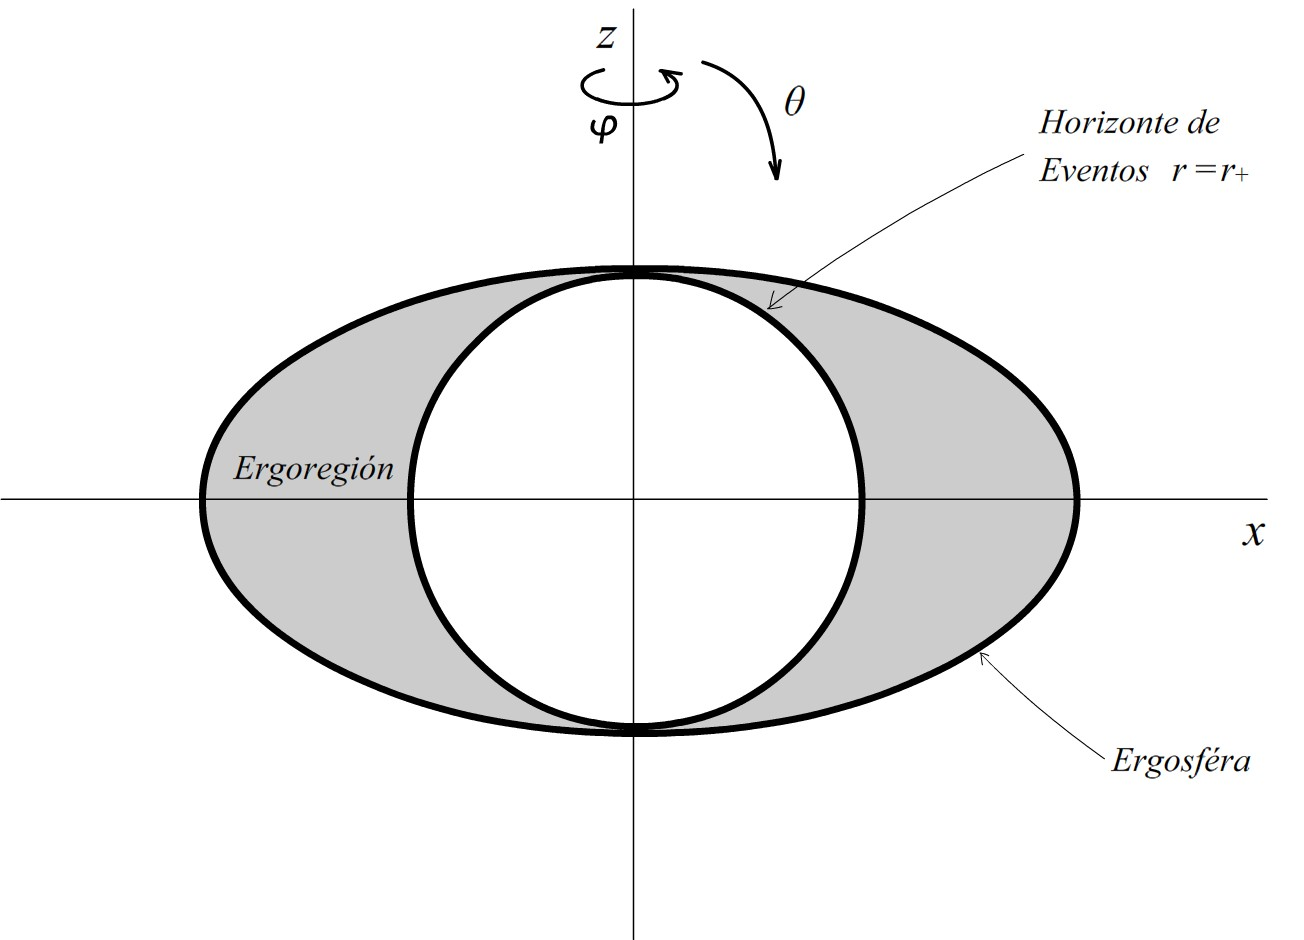
\includegraphics[scale=0.75] {figures/fig40.jpg}
				\end{figure}
			\end{center}	
        \end{frame}
  
     \begin{darkframes}
     	
        \begin{frame}{Dragging of inertial frames}
       	\framesubtitle{Case II: $M>a$}
            Photons moving in the equatorial plane
	$$ds^{2}= 0 = g_{tt} dt^{2} + 2g_{t\varphi} dt d\varphi + g_{\varphi\varphi} d\varphi^{2}$$
    		\pause
            The velocity of the photons is
            $$\frac{d\varphi}{dt}=-\frac{g_{t\varphi}}{g_{\varphi\varphi}}\pm\sqrt{\left(\frac{g_{t\varphi}}{g_{\varphi\varphi}}\right)^{2}-\frac{g_{tt}}{g_{\varphi\varphi}}}$$
        \end{frame}
        
        \begin{frame}{Dragging of inertial frames}
       	\framesubtitle{Case II: $M>a$}
            The velocity of the photons at the ergosphere is
            \begin{equation*}
            \left.\frac{d\varphi}{dt}\right|_{r=r_{e}}=\left\{ \begin{array}{c}
            \frac{a}{Mr_{e}+a^{2}\sin^{2}\theta}\\
            0
            \end{array}\right.
            \end{equation*}
        \end{frame}
    
    \subsection{Motion of particles and the Penrose's Process}
        \begin{frame}{Conserved Quantities for particle motion}
       	\framesubtitle{Case II: $M>a$}
            Energy
            $$E=-\xi^{\mu}p_{\mu}=-\xi^{t}p_{t}$$
            \pause
            $$E=-m\frac{dt}{d\tau}g_{tt}-m\frac{d\varphi}{d\tau}g_{t\varphi}$$
            \pause
            Angular Momentum
            \footnotesize
            $$L=-\left[\frac{a\sin^{2}\theta\left(r^{2}+a^{2}-\Delta\right)}{\varrho}\right]m\frac{dt}{d\tau}+\left[\frac{\left(r^{2}+a^{2}\right)-\Delta a^{2}\sin^{2}\theta}{\varrho}\right]\sin^{2}\theta m\frac{d\varphi}{d\tau}$$
        \end{frame}
        
        \begin{frame}{Penrose's Process}
       	\framesubtitle{Case II: $M>a$}
           Energy\\
           \bigskip
           
           $E=-\xi^{\mu}p_{\mu}>0$: Outside the ergosphere\\
           \bigskip
           \pause
           
           $E=-\xi^{\mu}p_{\mu}<0$: Inside the ergosphere
        \end{frame}
        
         \begin{frame}{Penrose's Process}
       	\framesubtitle{Case II: $M>a$}
           Consider a system composed by two particles initially in the asymptotic region and moving towards the
black hole.\\
\pause
\bigskip

Let $p_{\mu}^{o}$ be the initial 4-momentum of the composed
system.\\
\pause
\bigskip

The initial energy is positive and given by
$$E^{o}=-\xi^{\mu}p_{\mu}^{o}$$
        \end{frame}
        
        \end{darkframes}
    
        \begin{frame}{Penrose's Process}
         \framesubtitle{Case II: $M>a$}
        	\begin{center}
				\begin{figure}
				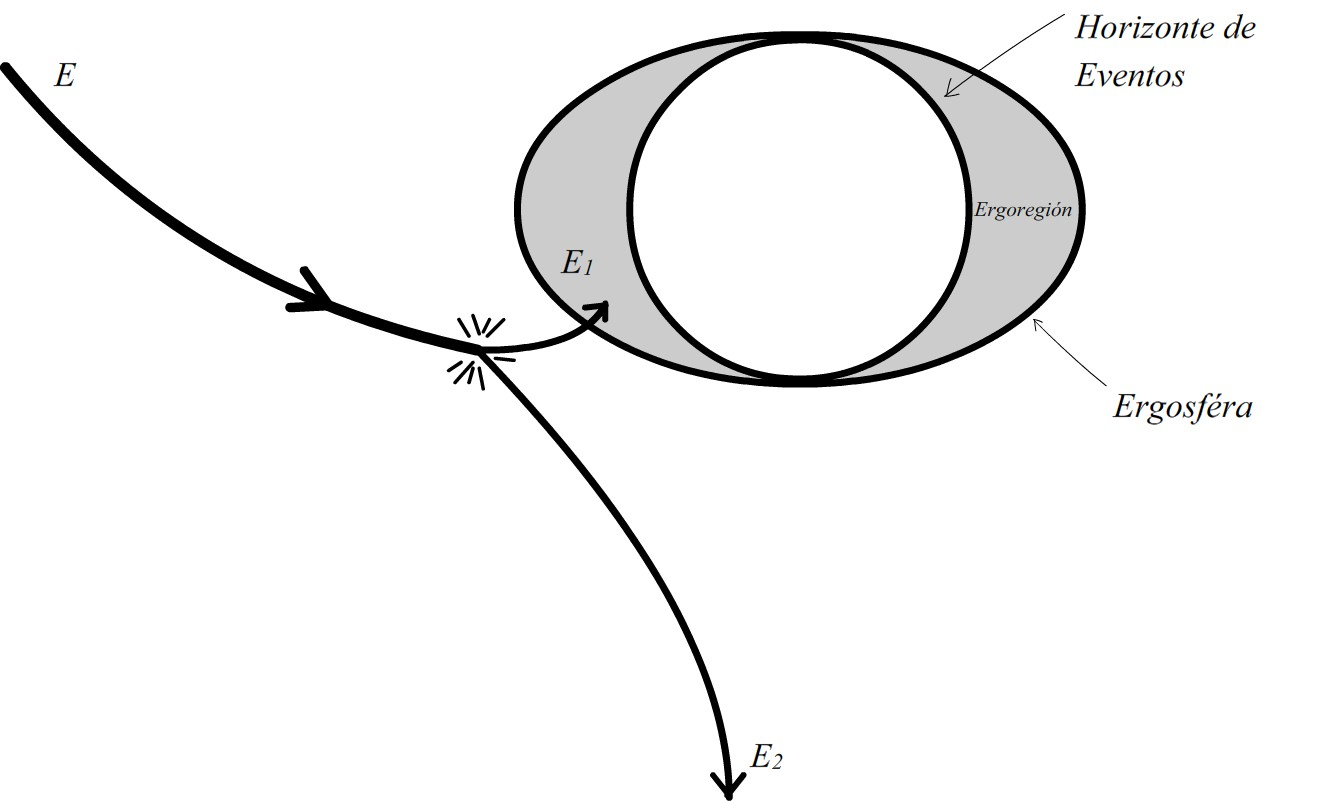
\includegraphics[scale=0.75] {figures/fig41.jpg}
				\end{figure}
			\end{center}	
        \end{frame}
  
     \begin{darkframes}
        
        
        \begin{frame}{Penrose's Process}
       	\framesubtitle{Case II: $M>a$}
           When the system is near the ergosphere, the system splits such that
one of the particles goes into the ergoregion while the other escapes
to the infinity.\\
\pause
\bigskip

The conservation of the 4-momentum gives
$$p_{\mu}^{o}=p_{\mu}^{1}+p_{\mu}^{2}$$
\pause
$p_{\mu}^{1}$ is the 4-momentum of the particle that goes into
the ergoregion and $p_{\mu}^{2}$ is the 4-momentum of the particle
that escapes.
        \end{frame}
        
        \begin{frame}{Penrose's Process}
       	\framesubtitle{Case II: $M>a$}
          	Contracting this equation with $\xi$, we obtain
            $$E^{o}=E^{1}+E^{2}$$
			\pause
            The energy of the particle inside is negative, $E^{1}<0$
            \pause
            \bigskip
            
            The energy of the particle that escapes is greater
than the initial energy:
$$E^{2}>E^{o}$$
i.e. the process extracts energy from the black hole.
        \end{frame}
        
        \end{darkframes}
    
        \begin{frame}{Penrose's Process}
         \framesubtitle{Case II: $M>a$}
        	\begin{center}
				\begin{figure}
				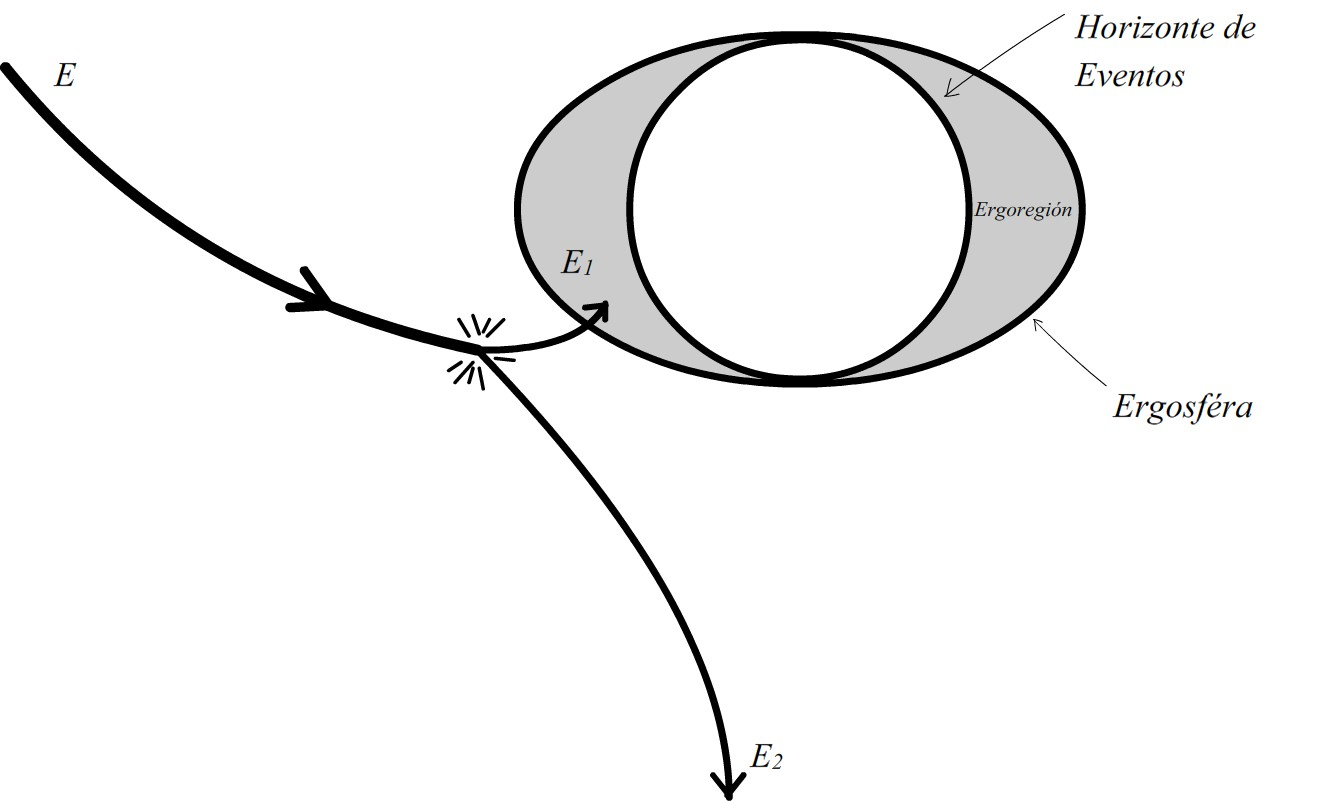
\includegraphics[scale=0.75] {figures/fig41.jpg}
				\end{figure}
			\end{center}	
        \end{frame}
  
     \begin{darkframes}
       
        \begin{frame}{Origin of the Extracted Energy}
       	\framesubtitle{Case II: $M>a$}
        $$\psi_{+}=\xi+\Omega\zeta$$
 		Is null (directed to the future) at the horizon $r=r_{+}$ and timelike outside this surface.
        \pause
        \bigskip
        
        $\psi_{+}^{\mu}p_{\mu}$ is negative or null outside the horizon,
        $$-\psi_{+}^{\mu}p_{\mu}\geq0$$
        \end{frame}
        
        \begin{frame}{Origin of the Extracted Energy}
       	\framesubtitle{Case II: $M>a$}
        Replacing $\psi_{+}$ and contracting
		$$E-\Omega L\geq0$$
        \pause
        $$L\leq\frac{E}{\Omega}$$
        \end{frame}
        
        \begin{frame}{Origin of the Extracted Energy}
       	\framesubtitle{Case II: $M>a$}
        For particle 1 (going inside the ergosphere)
        $$L^{1}\leq\frac{E^{1}}{\Omega}$$
        Since $E^{1}<0$, the angular momentum of this
particle is negative,
		$$L^{1}<0$$
        \pause
        The particle that goes inside diminishes the total angular momentum of the black hole, giving the energy extracted by the Penrose process.
        \end{frame}
        
        \begin{frame}{Limit for the Extraction of Energy}
       	\framesubtitle{Case II: $M>a$}
        Once we have extracted an amount of energy $E^{1}$, the black hole reaches, after some appropriate period of time, a new state of equilibrium in which its new mass is $M+\delta M$ and its new angular momentum is $J+\delta J$, where
        \begin{eqnarray*}
        \delta M & = & E^{1}\\
        \delta J & = & L^{1}
        \end{eqnarray*}
        \end{frame}
        
        \begin{frame}{Limit for the Extraction of Energy}
       	\framesubtitle{Case II: $M>a$}
        The relation between these quantities is as given above,
        $$\delta J\leq\frac{\delta M}{\Omega}$$
        \pause
        or
        $$\delta J\leq\frac{2M\left[M^{2}+\sqrt{M^{4}-J^{2}}\right]\delta M}{J}$$
        \end{frame}
        
        \begin{frame}{Limit for the Extraction of Energy}
       	\framesubtitle{Case II: $M>a$}
        $$\delta J\leq\frac{2M\left[M^{2}+\sqrt{M^{4}-J^{2}}\right]\delta M}{J}$$
        \pause
        $$\delta\left[M^{2}+\sqrt{M^{4}-J^{2}}\right]\geq0$$
        \end{frame}
        
        \begin{frame}{Area of the Event Horizon}
       	\framesubtitle{Case II: $M>a$}
        Area of the Event Horizon
      	$$A_H = \int_{0}^{\pi}\int_{0}^{2\pi} \left[\sqrt{\left|g_{\theta\theta}g_{\varphi\varphi}\right|} \right]_{r = r_{+}}d\theta d\varphi$$
        \pause
        $$A_H = 8\pi\left[M^{2}+\sqrt{M^{4}-J^{2}}\right]$$
        \end{frame}
        
        \begin{frame}{Limit for the Extraction of Energy}
       	\framesubtitle{Case II: $M>a$}
        $$\delta\left[M^{2}+\sqrt{M^{4}-J^{2}}\right]\geq0$$
        \pause
         $$\delta A_H\geq0$$
        \end{frame}
        
        \begin{frame}{Kerr Black Hole Singularities}
            $$r_{\pm}=M\pm\sqrt{M^{2}-a^{2}}$$
    	\end{frame}
       
        \begin{frame}{Case III: $M=a$}
            \begin{itemize}
            \item Extremal Kerr's metric: $M=a$ 
            \pause
            \item $r_{+}=r_{-}=M$ 
			$$\Delta=\left(r-M\right)^{2}$$
            \end{itemize}
        \end{frame}
        
        \begin{frame}{Eddington-Finkelstein's coordinates}
       		\framesubtitle{Case III: $M=a$}
           	Eddington-Finkelstein's coordinates

           	\begin{eqnarray*}
           	dv & = & dt+\frac{\left(r^{2}+M^{2}\right)}{\left(r-M\right)^{2}}dr\\
           	d\chi & = & d\varphi+\frac{M}{\left(r-M\right)^{2}}dr
           	\end{eqnarray*}
          	\pause
          	\footnotesize
          	\begin{eqnarray*}
  			ds^{2} & = & -\frac{r^{2}-2Mr+M^{2}\cos^{2}\theta}{\varrho}dv^{2}+2dvdr-\frac{4M^{2} r \sin^{2}\theta}{\varrho}dvd\chi\\
   				&  & -2M\sin^{2}\theta drd\chi+\varrho d\theta^{2}+\frac{\left(r^{2}+M^{2}\right)^{2}-\left(r-M\right)^{2}M^{2}\sin^{2}\theta}{\varrho}\sin^{2}\theta d\chi^{2}
          	\end{eqnarray*}
        \end{frame}
        
        \begin{frame}{Killing Vectors}
       		\framesubtitle{Case III: $M=a$}
            $$\xi=\frac{\partial}{\partial v}$$
 			$$\zeta=\frac{\partial}{\partial\chi}$$
        \end{frame}
        
        \begin{frame}{Killing Horizon}
       		The hypersurface $r=M$ is a degenerate Killing horizon (i.e. with
            $\kappa=0$) of the vector
            $$\psi=\xi+\Omega\zeta$$
            \pause
            Angular velocity:
            $$\Omega=\frac{a}{2M^{2}}=\frac{1}{2M}$$
        \end{frame}

  \end{darkframes}

         \begin{frame}{Carter-Penrose Diagram. $\theta=0$ and $\theta= \frac{\pi}{2}$}
      \framesubtitle{Case III: $M=a$}
        	\begin{center}
				\begin{figure}
				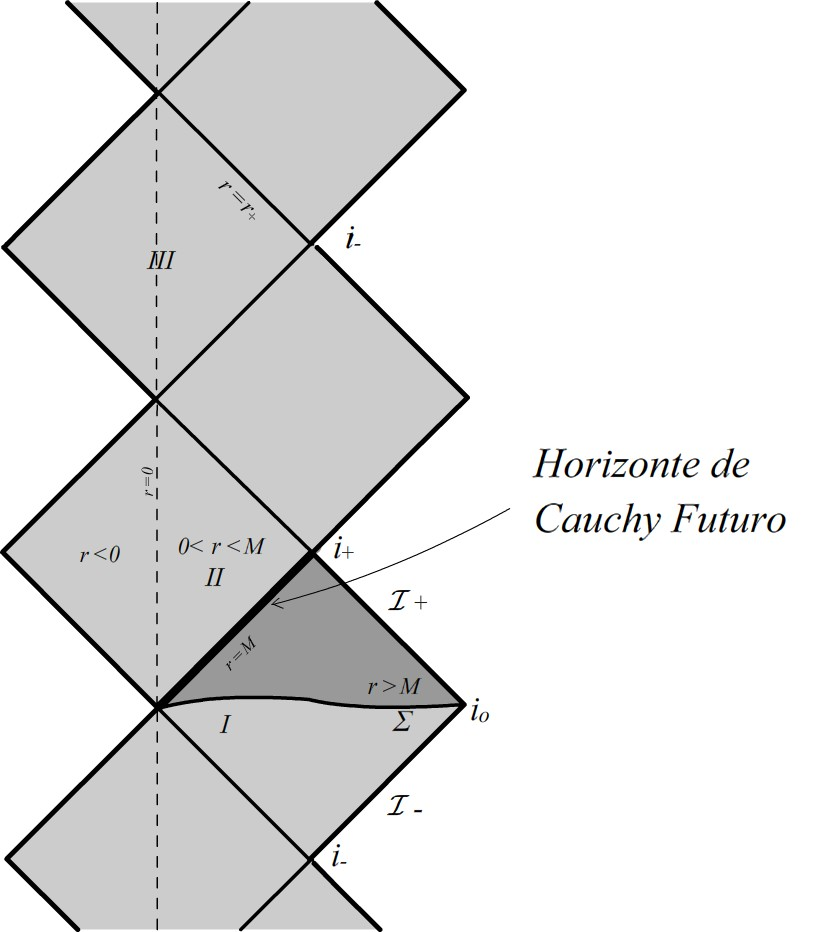
\includegraphics[scale=0.75] {figures/fig42.jpg}
				\end{figure}
			\end{center}	
        \end{frame}
        
  \begin{darkframes}
        
  		\begin{frame}{Next Lecture}
        	\Large
			{06. Black Holes Astrophysics}
		\end{frame}
  
  \end{darkframes}
\end{document}
